\chapter{FPGA Firmware}
\label{ch:firmware-design}
\setsvg{svgpath=./img/firmware/}
\graphicspath{{./img/firmware/}}

This Chapter details the design, implementation and testing of the FPGA firmware. Testing involves both simulating using data path as well putting the firmware on the physical FPGA, sending input RF signals to it and analysing the output of the FPGA's DSP.

\section{Hardware Specifications}

\begin{figure}
  \centering
  \includegraphics[width=\textwidth]{roach-photo}
  \caption{Photo of the ROACH board and ADCs. Bottom: Two Atmel AT84AD001B dual ADC cards with SMA connectors going in to them and connected via Z-DOK to the ROACH board. Bottom right: ADC clock synthesiser feeding into power splitter which in turn clocks each ADC board in phase. Top: main ROACH board. The Virtex-5 is under the blue fan. To its left is the ROACH's DRAM module. To the right of the fan is the PowerPC with its DRAM module.}
  \label{fig:firmware:roach-photo}
\end{figure}

As discussed in the user requirements, the FPGA processing board that should be use is the same which is used by the SKA: the Reconfigurable Open Architecture Computing Hardware (ROACH)\footnote{\url{https://casper.berkeley.edu/wiki/ROACH}} board. This board has a Xilinx Virtex-5 FPGA on it, with connectors for Z-DOK+ cards which will be used for ADCs and a DDR2 DRAM connector for high volume\footnote{Compared to the Virtex-5's on-chip storage} data storage. There is a PowerPC subsystem on the ROACH running Linux which provides a 1 Gbps Ethernet interface for programming and data readout from the memory of the FPGA. The PowerPC runs a daemon called tcpborphserver which speaks the KATCP protocol used to interact with the ROACH. There are other blocks on the ROACH board as well, but the ones listed here will be the ones utilised in this project.

There are various ADC cards compatible with the ROACH. The ones which were made available for this project are iADC cards. Each card has an Atmel/e2V AT84AD001B 8-bit dual ADC chip on it. It's designed for I/Q sampling but can be configured to sample both channels in phase; exactly what's needed here. The clock speed can be up to \SI{1}{\giga\hertz} and must be externally supplied. The ADC feeds the clock signal through to the FPGA along with the sampled data with a demux factor of 4:1 meaning that for every 4 ADC clock cycles and 4 samples, the FPGA gets one clock cycle with all 4 samples on the ADC data bus. This implies that the FPGA will run at exactly a quarter of the speed the ADC runs at, and needs to be able to handle 4 samples per channel times 4 channels = 16 samples every clock cycle.

The clock source is a Valon 5007 dual synthesiser which is USB programmable from \SI{137}{\mega\hertz} to \SI{4400}{\mega\hertz}. Both ADCs need to be clocked exactly in phase so the Valon is fed into a Mini-Circuits ZESC2-11+ power splitter which has a low phase imbalance.

The ROACH board with connected ADCs is shown in \Cref{fig:firmware:roach-photo}. All of the components are in a metal case for RF shielding, although the cover has been removed for the photo.


\section{Firmware Development Toolchain}
There are a few components necessary to get development for the ROACH working. They're briefly listed here and detailed more in \Cref{appendix:roach-development}.\\

Xilinx ISE 14.7 is needed for synthesising (compiling) HDL files to FPGA bitfiles. This proprietary tools is maintained by Xilinx and made available through the SKA. As well as this key task of compilation it also has peripheral tools for debugging and optimisation which proved useful for getting the design to meet timing. More info in \Cref{appendix:roach-development}. Although it also works on Debian/Ubuntu systems, ISE is most stable and only officially supported for RHEL. As such as CentOS system was used for FPGA development work as it's mostly the same as RHEL at the binary interface level.\\

Matlab R2012B with Simulink was installed, along  with the mlib-devel plugin. The majority of the design work for ROACH done in this project is done at the block diagram level in Simulink. There is a plugin called mlib-devel which defines the Simulink interface for the Xilinx cores, as well as containing HDL code for ROACH specific hardware such as ADC cards, DRAM interface and PowerPC control bus. This naturally includes the net definitions for the components on the ROACH board.

The mlib-devel plugin was originally created by CASPER, now contributed to extensively by the SKA. It contains a multitude of highly useful DSP blocks which are built on top of the Xilinx cores which can be wired up in Simulink. These include range from relatively simple blocks like edge detectors to very complex ones like real-time FFT blocks and polyphase filterbank blocks. Additionally, blocks for interfacing with hardware like ADCs, memory, shared registered and generic IO are included. It was necessary for this project to update some blocks during this project, hence a clone of this mlib-devel repo was created\footnote{\url{https://github.com/jgowans/mlib_devel}}.


\section{Design}
There are a number of subsystems developed for the FPGA which will be discussed here. Most of these subsystems required extensive development, testing and tweaking. The full design is shown in \Cref{fig:firmware:full-design}. It may be difficult to see all of the detail of the design, but the purpose of the figure is to give an indication of the structure, layout and data flow in the FPGA. The following subsections discuss the purpose of the key blocks in the design. A more detailed look at the composition and structure of the some of the blocks can be found in \Cref{appendix:roach-development}. That Appendix also discusses the challenges that were encountered during the FPGA design, and the optimisations that were done to get it working.

\afterpage{%
  \clearpage% 
  \begin{landscape}
    \thispagestyle{empty}
    \begin{figure}
      \vspace{-4em}
      \centering
      \makebox[\textwidth][c] {
        \includegraphics[width=1.22\paperwidth,center]{full-design-a4-no-sim-out.pdf}%
      }%
      \caption{Full FPGA design containing frequency and time DSP paths and control logic.}
      \label{fig:firmware:full-design}
    \end{figure}
  \end{landscape}
}

\subsection{ADCs}
The yellow blocks on the left represent the two dual ADCs. These \(2 \times 2\) channels will be referred to as channel 0, 1, 2 and 3. Each ADC has \(2 \times 4 = 8\) 8-bit buses for the signed integer samples that are clocked in every clock cycle. As mentioned earlier the FPGA runs at a quarter of the ADC clock cycle hence the ADC presents 4 samples per clock cycle.  Also included are logic lines that indicate clipping. For simulation purposes, normal Simulink signal source blocks can be connected to the ADC, allowing the construction of arbitrarily complex input signals. The example shows a simple chirp connected. The output from the ADCs fans out to two distinct signals paths: a frequency domain path and a time domain path. These are now explored.

\subsection{Frequency domain signal path}
The frequency domain path starts with an FFT block, the first big green one,  which performs real time FFTs on the data from the ADCs. Although it's one block it does four distinct Fourier transforms under the hood, one for each of the ADC channels. It's an 11 stage FFT meaning that it does \(2^{11} = 2048\) points. It has an optimisation for real-valued signals in that it only output the positive half of the frequency spectrum to save bandwidth. The FFT has been configured to do full bit growth, meaning that every stage another bit of data is added to the bus size. This means that weak signals will be preserved as no bits are thrown away. This is at the expense of significant data growth: each channel outputs two 36-bit complex numbers every clock cycle.

FFT output is fed into the second big green block, the Cross Multiplier. This does \({4 \choose 2} = 6\) cross multiplications, one for each baseline, as well as one additional for the autocorrelation of channel 0 to serve as a spectrum analyser. These are referred to as 0x0, 0x1, 0x2, 0x3, 1x2, 1x3 and 2x3. The cross multiplication involves breaking the signal up into its real and imaginary component, taking the complex conjugate of one of the signals by inverting the sign of its complex component and then doing complex multiplication. For each pair of signals signals \(A\) and \(B\) where \(A = (a + ib)\) and \(B = (c + id)\) the FPGA will do \(C = A\overline{B} = (ac + bd) + (bc - ad)i\). The cross multiplier does not throw any bits away meaning that the signals go from a \(2 \times 36 = 72\) bit complex numbers to 148 bits per channel.

The cross correlation signals then go to the white Accumulators block. As discussed in Chapter 3, the cross correlations will be accumulated (aka: integrated) a number of times in order to allow weak signals to stand out of the noise. The accumulation length is runtime programmable via a control register which will be discussed more later. The accumulator works by using FPGA BRAM to produce a delay, and a DSP48E to add the new signal to the current one. The length of the BRAM is the number of points in the FFT spectrum, 2048. The accumulators allow signal growth from 74 bits per complex number to 96 bits. This implies a minimum of \(\approx 4\) million accumulations when the signals are full scale, although typically this can be orders of magnitude more as the system does not run with full scale input; it's too dangerous the keep the ADCs at max power.

Each accumulated correlation value is wired to its own BRAM snapshot block, the array of small green blocks on the right. Once sufficient accumulations have been run, the snapshot blocks are triggered to take a snapshot of the correlation spectrums. The snapshots then record the full accumulated correlation spectrum of a channel, now 128 bits wide per frequency channel per correlation pair, to shared BRAM memory. This memory can then be read out from the FPGA via the PowerPC over Ethernet.

\subsection{Time domain signal path}
This path is comparatively simpler than the frequency domain path, seeing as the correlations are not being done on the FPGA, and seeing as accumulation is not applicable for time domain DF. 

There are two main blocks for the time domain path, which are at the bottom of the FPGA design. First is the impulse detector. This takes in the raw ADC data from channel 0 and runs a rolling sum filter which provides the sum of the last \(N\) samples where \(N\) is some runtime programmable number, typically between 10 and 1000 samples. If the rolling sum goes above a runtime programmable threshold the impulse detector considers an impulse to be present. It then records the raw time domain data of all 4 channels for as long as the impulse is present, plus some additional buffer at the start and end of the pulse.  The snapshot is stored by the green block at the bottom, the off-chip DRAM module. The starting buffer is attained by feeding a delayed version of the raw signal to the DRAM interface. The DRAM module was chosen as it can store a large amount of data, allowing multiple milliseconds of raw data to be stored if desired. Typically only a few microseconds of data is necessary to store an impulsive signal. As well as triggering the snapshot, the impulse detector will also store the length of the impulse which it detected so that the computer knows much data to read out from the DRAM module when it wants the data. The DRAM data is also accessible through the PowerPC over Ethernet.

\subsection{Control and Monitoring}
The FPGAs runtime configuration and status can be interacted with via shared memory accessible in the address space of the PowerPC. This memory manifests as as words of data registers on the FPGA. Slices of these registers are wired to different parts of the FPGA logic to dynamically change it in the case of writable memory, or to get status info in the case of readable memory. The registers are the yellow blocks dotted around the design. Following are a few control and monitoring functions. The description of what they do also indicates more about how the design works.
\begin{itemize}
  \item Integers for accumulation length, impulse detector rolling filter length and impulse detector setpoint. These are all separate 32 bit registers for runtime configuration of these values.
  \item Impulse detector arm. The impulse detector will only write a snapshot to DRAM if its threshold is breached while the arm latch is high. The latch is cleared when a snapshot is detected, and can be set again by the computer once the snapshot has been read out. The reason for this is to prevent the race condition where a new snapshot could partially overwrite an earlier one which is busy being read out by the computer.
  \item Snapshot trigger gate. Similar to the reasoning behind the impulse detector arming, this gate to all of the snapshot trigger blocks exists to prevent a new accumulated spectrum from being written on top of one that is being read out. The computer will gate the trigger while it's busy reading the snapshot blocks, and clear the gate once the readout is complete.
  \item Rolling sum level. This is the current value of the rolling sum filter. By watching the value of the filter for some time, an informed decision can be made about where to put the setpoint for the impulse detector. Typically this would be a few standard deviations above the mean. Setting its value is a trade off between false positives and false negatives.
  \item Impulse length. The impulse detector records how long the impulse goes on for. The computer can poll this value to see how much data needs to be read from DRAM. By reading only the minimum data, the readout is faster and the time domain cross correlation is more accurate.
  \item Overflow status latch and reset. The various parts of the system which can overflow feed latched version of their overflow status lines into a register. Then, whenever a snapshot is read out the overflow register is examined as well so see if the data should be treated as valid or not. There are multiple bits so it can be seen which part of the system overflowed and configuration can be adjusted to remediate this overflow. For ADC overflow this would be adding analogue attenuators. For accumulation overflow this would be reducing the accumulation length. For FFT overflow this would be changing the shift schedule. As well as going a register to be read out by the computer, this overflow latch is also fed to GPIO register which drives an LED mounted on the ROACH case so that should any overflow happen it will immediately light the LED to inform the operator. The computer can acknowledge the occurrence of overflow by pulsing a reset line which will clear the latch.
  \item Manual sync pulse. Data is streamed into the FFT block and frequency channels come out in order which eventually need to be stored in snapshot memory, lowest numbered channel at the start and highest channel at the end. As such, something needs to keep track of which channel is the first one. The sync pulse achieves this by resetting the FFT, and the FFT will then output the sync pulse at the same clock cycle as channel 0. This sync pulse is then propagated through the multipliers and in to the accumulators, which ensures that the start of an accumulation is in phase with the start of a spectrum. This sync line is pulsed by the computer when it connects to initialize the data path.
  \item Accumulation counter. Every time an accumulation is completed and a new one started, this counter increments. The computer can use this to know when it's time to read out a new spectrum and also to ensure it's keeping up and reading out all snapshots.
  \item FFT shift schedule. Sets which phases the FFT should shift data down by 1 bit and when it should allow bit growth. It ended up not being needed as it was possible to fit a full bit growth FFT on to the design. However, should a longer FFT or other additional logic be needed in future, it will be necessary to shrink the width of the data path and then use a shifting FFT.
\end{itemize}

\section{Simulation}
\begin{figure}
  \begin{subfigure}{\textwidth}
    \centering
    \includegraphics[width=0.8\textwidth]{impulse}
    \caption{Periodic \SI{1}{\micro\second} impulse at half of the power of the noise}
  \end{subfigure}
  \begin{subfigure}{\textwidth}
    \centering
    \includegraphics[width=0.8\textwidth]{noise}
    \caption{Additive Gaussian white noise}
  \end{subfigure}
  \begin{subfigure}{\textwidth}
    \centering
    \includegraphics[width=0.8\textwidth]{impulse-plus-noise}
    \caption{Sum of impulse and noise. Impulse is not distinguishable by eye.}
  \end{subfigure}
  \begin{subfigure}{\textwidth}
    \centering
    \includegraphics[width=0.8\textwidth]{filter}
    \caption{Output of moving sum filter. Additional noise power now clearly visible}
  \end{subfigure}
  \caption{Simulink simulation of how filter can detect impulse even below noise floor.}
  \label{fig:firmware:impulse-detection-simulation}
\end{figure}
As the design is created in Simulink, the extensive simulation capabilities it provides can be used to validate that the design should behave as intended. Simulation was used throughout the development process, for both the time and frequency domain signal path. For example, for the frequency domain path a repeating correlated chirp signal with a defined start and end frequency would be injected in the input, and the snapshot blocks would be examined to ensure that there was a flat power spectrum between those frequencies. For the time domain path, short impulses in the presence of noise were simulated, and the output of the rolling average filter monitored to ensure that it correctly detected a rise in power. An example of this is shown in \Cref{fig:firmware:impulse-detection-simulation}. This example has the extreme case where the impulse is actually smaller than the additive noise, yet the filter is able to detect it and could trigger a capture of it.

\section{Design compilation}
Over the course of this research, the design developed from being a simple two-antenna time domain data collector to the full four-antenna time and frequency domain DSP subsystem described here. The full design is very large, consuming more than 95\% of the available logic on the FPGA. Numerous optimisation were necessary to get it to fit which are detailed more in \Cref{appendix:roach-development}.

Part of the compilation process involves defining the clock speed at which the FPGA should operate. The Xilinx tools then move logic around to ensure that all signals can propagate and be valid in the necessary time. Hence faster speeds are more difficult to compile as it's more likely a path will not meet timing. The timing value that proved reliable for this design was \SI{200}{\mega\hertz}. This implies an ADC clock speed of \SI{800}{\mega\hertz}. The ADCs have a maximum clock speed of \SI{1000}{\mega\hertz} so this speed is fine for them. 

The ADC's \SI{800}{\mega\hertz} sample rate implies a Nyquist frequency of \SI{400}{\mega\hertz} which explains why \SI{400}{\mega\hertz} has been used extensively in the previous sections for DF algorithm simulations and antenna design.

\section{Lab Tests}
In order to validate that the FPGA subsystem was working as expected, a hardware setup was created in the lab to emulate the sort of signals which the DF system would see in the field. The setup contained signal sources for both strong impulsive signals, as well as weak narrow band tone signals. The impulses and tones were split and fed to all ADCs. As well as getting the correlated signals, uncorrelated noise was added, allowing more accurate tests ensuring that the correlation and accumulation part of the DSP path could extract weak signals from noise. The physical setup in the lab is shown in \Cref{fig:firmware:lab-setup-photo} with a diagram of the configuration in \Cref{fig:firmware-lab-setup-diagram}. 

This hardware rig was used during development in conjunction with the Simulink simulations to ensure that the running design was operating as intended. 

For the time domain path the tests involved arming the time domain capture, then manually triggering a one-shot impulse. The system successfully detected the impulse and captured it on all four channels, was well as its length with some start and stop buffer to DRAM. This signal could then be read out.

The frequency domain path tests involved producing a tone at a certain frequency and ensuring that accurate phase difference as seen by each input was seen after accumulation. The expected phase was set by feeding different cable lengths from the splitter to the ADCs. Two situations were tested, one where all cables were of equal lengths hence expecting to see \SI{0}{\degree} phase shift between all baselines. The other test was where one cable was longer than the rest, hence expecting some of the baselines to see a phase shift while others to be in phase. The expected phase shift was checked by measuring the cables on a network analyser. These tests were done at different SNR levels to quantify not only that the observed phase shift was present but also how performance changed with SNR level and with accumulation length. Results for SNR levels of 0.1, 0.01 and 0.001 are shown in Figure 5.6. Note that these SNR levels are for the noise power in just the channel of the signal, not total noise power. Total noise power is order of magnitudes higher as the white noise has power across the whole spectrum. These results show that the system is behaving as expected in two key ways. First, in general, error diminishes as more samples are accumulated. Second, the higher the SNR the faster the lower the faster the error drops off. Based on these results we can say that the system is able to operate all the way down to SNR levels of 0.01 provided integration time can span hundreds of thousands of samples, or a few seconds.

\begin{figure}
  \centering
  \includegraphics[width=\textwidth]{lab-setup-photo-labeled-resized}
  \caption{Equipment setup in the lab. Top to bottom: ROACH; four noise sources; RF splitters, combiners and attenuators; RF board with amplifiers and filters; impulse generator; trigger and gate for impulse generator; signal generator for narrow band signals}
  \label{fig:firmware:lab-setup-photo}
\end{figure}
\begin{figure}
  \centering
  \includegraphics[height=\textheight]{lab-setup-diagram}
  \caption{Diagram showing how the various components in \Cref{fig:firmware:lab-setup-photo} are connected together.}
  \label{fig:firmware-lab-setup-diagram}
\end{figure}

\afterpage{%
\thispagestyle{empty}
\begin{figure}
  \vspace{-4em}
  \begin{subfigure}{\textwidth}
    \centering
    \includegraphics[width=0.7\textwidth]{integration-vs-error-0x1-2}
  \end{subfigure}
  \begin{subfigure}{\textwidth}
    \centering
    \includegraphics[width=0.7\textwidth]{integration-vs-error-0x01-2}
  \end{subfigure}
  \begin{subfigure}{\textwidth}
    \centering
    \includegraphics[width=0.65\textwidth]{integration-vs-error-0x001-2}
  \end{subfigure}
  \caption{Plots for integration length vs output error tests in SNRs of 0.1, 0.01 and 0.001. Each line on the graph is an iteration of the test.}
  \label{fig:firmware:phase-error-measurement-plots}
\end{figure}
}


\section{Summary}
This Chapter has first discussed the DSP signal paths in the FPGA design, including the frequency domain cross correlation and accumulation path, and the time domain rolling sum filter and impulse detection paths. It also discussed the control and monitoring blocked used to interface with a computer. Next, it was shown how the design has been tested and verified, using both Simulink simulations and a hardware setup in the lab. The hardware setup has RF sources for impulses, tones, and uncorrelated noise. The performance of the system was as expected, being able to detect and capture impulses, as well as measure the phase of tones which were well below the noise floor.
